\begin{figure*}

  \begin{panel}{(b)}{\textwidth}
    \vspace{4mm}
    \tikzsetnextfilename{figure_1_model}
    \begin{tikzpicture}

  % parameters
  \node[var] (n) {\n};
  \node[var,below of=n] (theta_T) {\parameterst};
  \node[var,below of=theta_T] (theta_E) {\parameterse};
  \node[var,below of=theta_E] (theta_C) {\parametersc};

  % hidden states
  \node[state,right=1cm] (z1) at ($(n)!.5!(theta_T)$) {\z{1}};
  \node[state,right=4mm of z1] (z2) {\z{2}};
  \node[state,right=1cm of z2] (zt) {\z{t}};
  \node at ($(z2)!.5!(zt)$) {$\cdots$};

  % observations
  \node[observation,right=1cm] (x1) at ($(theta_E)!.5!(theta_C)$) {\x{1}};
  \node[observation,right=4mm of x1] (x2) {\x{2}};
  \node[observation,right=1cm of x2] (xt) {\x{t}};
  \node at ($(x2)!.5!(xt)$) {$\cdots$};

  % plates
  \begin{pgfonlayer}{background}
    \node[plate,fit=(z1)(zt)] (hidden) {};
    \node[plate,fit=(x1)(xt)] (observed) {};
  \end{pgfonlayer}

  % dependencies
  \draw[arrow] (n) to (hidden);
  \draw[arrow] (theta_T) to (hidden);
  \draw[arrow] (theta_E) to (observed);
  \draw[arrow] (theta_C) to (observed);
  \draw[arrow] (z1) to (x1);
  \draw[arrow] (z2) to (x2);
  \draw[arrow] (zt) to (xt);
  \draw[arrow] (z1) to (z2);
  \draw[arrow,shorten <=20] (z2) to (zt);
  \draw[shorten >=22] (z2) to (zt);

  % annotation
  \node[below of=observed] {$p(\trace|\n,\parameterst,\parameterse,\parametersc)$};

\end{tikzpicture}
%
  \end{panel}
\end{figure*}

\begin{figure*}
  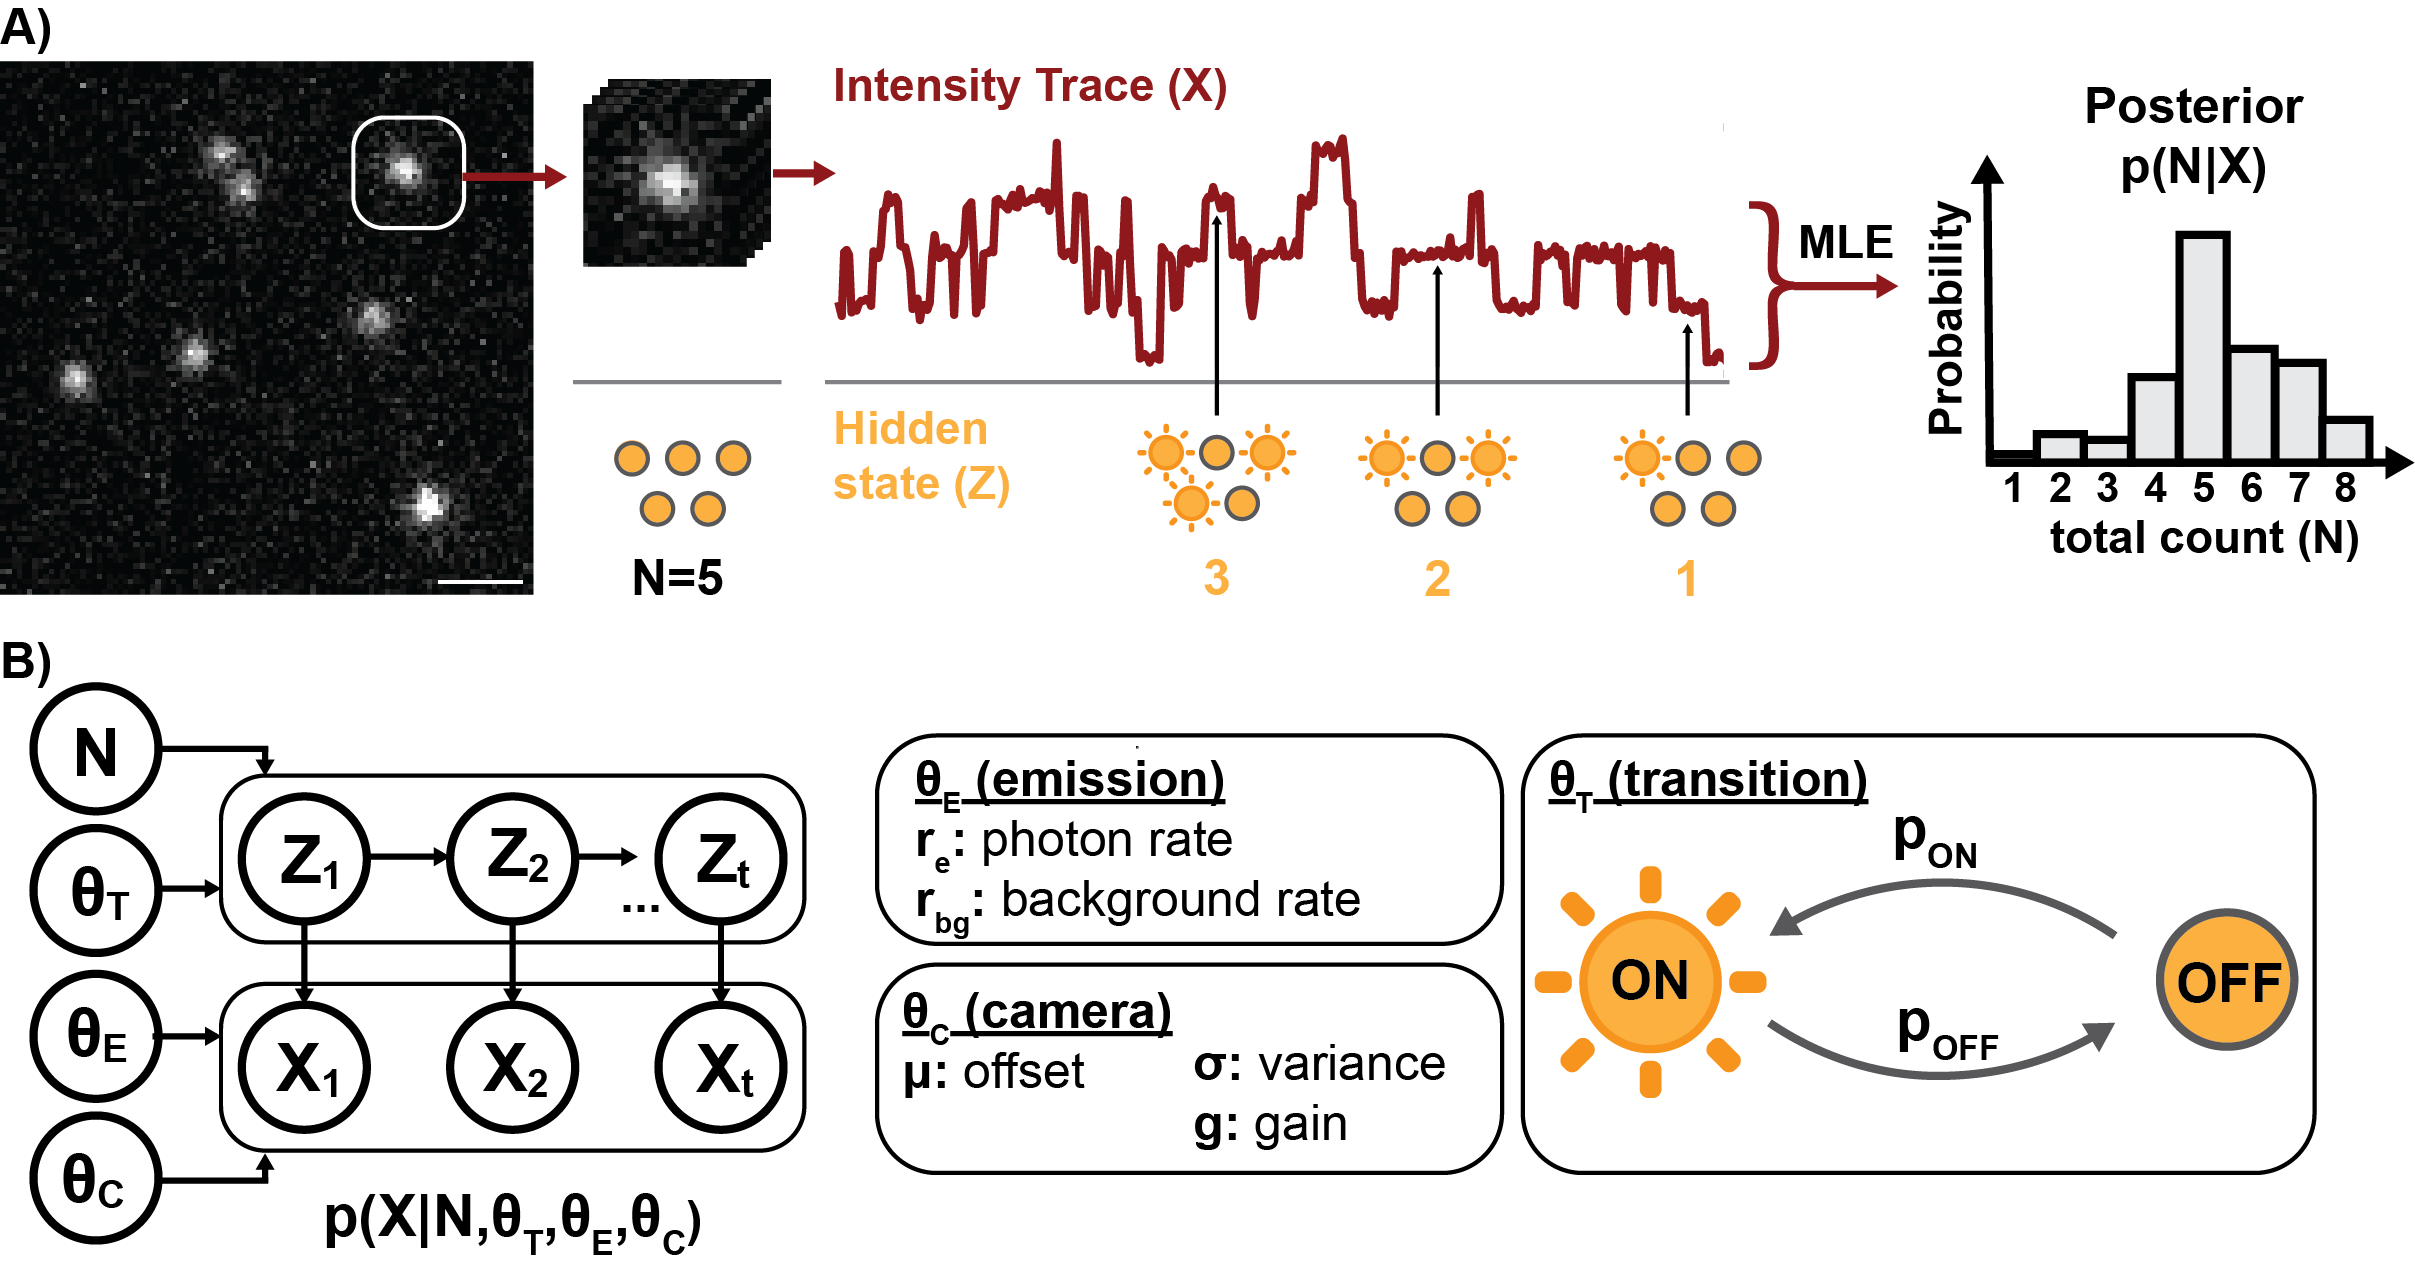
\includegraphics[width=\linewidth]{figures/placeholders/figure_1_overview.png}
  \caption{A) Overview of the blinx method (scale bar: 1 $\mu$m) B) blinx is based on a Hidden Markov Model who's parameters are optimized to build the final posterior
  distribution}
  \label{fig:method:overview}
\end{figure*}
